\chapter{Displays}
\chaplabel{displays}

\section{Introduction}
Adding a display to a device allows much more information to be shared from the device to the user than 
just using LEDs or buzzers. There are several types of displays that are commonly used in the embedded systems 
world. 

\subsection{LCD}
The most common is a Liquid Crystal Display (LCD). Most of the computer monitors and computers are LCD. This 
technology gives good contrast, fast response (which gamers like), and minimal burn in. Old CRT displays had 
to have screensavers so that whatever was usually showing on the display wouldn't be there permanently. 
Thankfully modern displays don't typically have this problem. LCDs do require a backlight. This determines
how bright the colors are. The pixels in the display just modulate how much of the backlight is showing.

At times you will find TFT displays. This stands for thin-film-transistor liquid-crystal display. They are 
a better version of LCD.

\subsection{eInk}
eInk displays are also available for embedded systems. These displays are of particular interest because they keep their 
display even when the power is turned off. This allows for very low power operations. The downsides are 
that they work off of reflected light so require special backlighting to be viewed at night and that 
they are very slow. A small display may take several seconds to refresh and some recommend not to update
them more than once every few minutes if possible.

\subsection{OLED}
The cool part about Organic Light Emitting Diode (OLED) displays is that  
instead of each pixel blocking the backlight to make the display like in LCDs, in 
OLED displays each pixel is an LED that emits light. This makes OLED displays very bright with very 
good contrast ratios. They also have fast response times. Some OLED displays will get dimmer with time. 
\href{https://www.adafruit.com/product/938}{Adafruit notes} that for their small 
OLED displays the dimming becomes noticeable after about 1000~hours of being on. This is 41.7~days, 
so after a year of continuous use, an OLED display might not be very bright.

\section{Pixel Layout}
The layout of pixels on a display can be thought of as a cartesian coordinate system with a couple 
minor differences. First, pixels take up space, so the indexing is between the lines rather than 
on the lines. Second, the +Y axis points downward as shown in Figure \ref{fig:pixels}. The units
for the coordinates is always pixels and the coordinates are always integers. 

Pixels can vary in size. This is important to keep in mind if you are trying to display something
with a specific size. Pixel size varies from display to display so read carefully if you want 
something to display a specific size.

\newcommand*{\xMin}{0}%
\newcommand*{\xMax}{6}%
\newcommand*{\yMin}{0}%
\newcommand*{\yMax}{6}%
\begin{figure}[!htb]
	\centering
	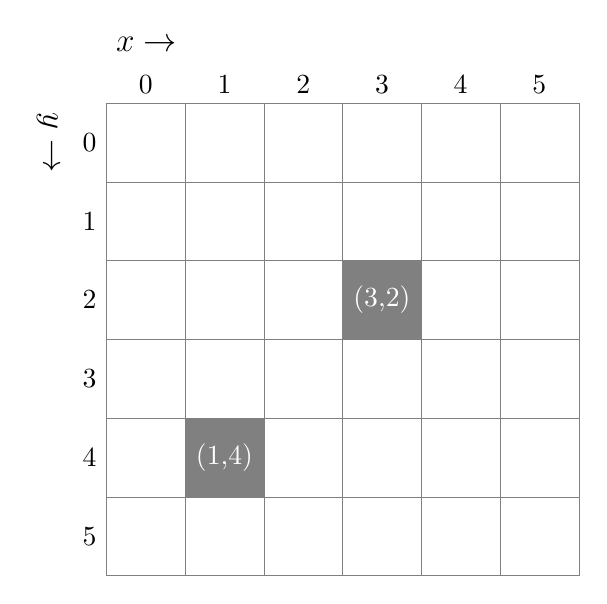
\begin{tikzpicture}

		\node[anchor=west] at (0,6.75) {\large$x\rightarrow$};
		\node[anchor=west,rotate=-90] at (-0.75,6) {\large$y\rightarrow$};

		\foreach \i in {\xMin,...,\xMax} {
			\draw [very thin,gray] (\i,\yMin) -- (\i,\yMax);
		}
		%https://tex.stackexchange.com/questions/36713/computing-in-the-list-of-a-tikz-foreach
		\foreach \i in {\xMin,...,\number\numexpr\xMax-1\relax} {
			\node[anchor=south] at (\i+0.5,\yMax) {$\i$}; 
		}
		\foreach \i in {\yMin,...,\yMax} {
			\draw [very thin,gray] (\xMin,\i) -- (\xMax,\i);
		}
		\foreach \i in {\yMin,...,\number\numexpr\yMax-1\relax} {
			\node[anchor=east] at (\xMin,\yMax - \i-0.5) {$\i$}; 
		}
		\fill [gray] (3,3) rectangle (4,4);
		\node[anchor=center] at (3.5,3.5) {\color{white}(3,2)};
		\fill [gray] (1,1) rectangle (2,2);
		\node[anchor=center] at (1.5,1.5) {\color{white}(1,4)};
	\end{tikzpicture}
	\caption{Pixels in a display occupy space are are referenced to the top left corner with the positive Y axis going down.}
	\label{fig:pixels}
\end{figure}

\section{Using the Display}
The display on the lab board is a 1.14" TFT display 240~pixels wide and 135~pixels high. 
Two libraries are required to use it:
\begin{enumerate}
	\item \lstinline@Adafruit_GFX.h@ - this is the generic graphics library
	\item \lstinline@Adafruit_ST7789.h@ - this is specific to our display
\end{enumerate}
An example that shows much of the available functionality can be found (once the libraries are installed)
at Examples $\rightarrow$ Adafruit ST7735 and ST7789 Library $\rightarrow$ graphicstest\_st7789. 
The following have to be defined to use a display:
\begin{enumerate}
	\item Width - how many pixels wide the display is 
	\item Height - how many pixels high the display is 
	\item Reset pin - Allows the microcontroller to reset the display
	\item CS - Chip Select, used by SPI to select the display when communicating
	\item DC - Data/Command pin used to determine the type of data being sent to the display
\end{enumerate}

An example of creating a display instance is as follows:\\
\lstinline@Adafruit_ST7789 tft = Adafruit_ST7789(TFT_CS, TFT_DC, TFT_RST);@

Some useful methods that can be called on the display object are:
\begin{enumerate}
	\item fillScreen - Fills the screen with the specified color. Usually used to clear the screen.
	\item setTextSize - sets the size of the text (usually 2-4)
	\item setTextColor - set what color the text should be. Some examples are 
	\begin{enumerate}
        \item ST77XX\_BLACK
        \item ST77XX\_BLUE
        \item ST77XX\_RED
        \item ST77XX\_YELLOW
    \end{enumerate}
	\item print/println - these act the same as they do when using Serial
	\item drawBitmap - draws a bitmap stored using PROGMEM or a canvas. It requires the following arugments
	\begin{enumerate}
		\item xpos - the x position for the image
		\item ypos - the y position for the image
		\item bitmap variable - the variables with the actual image
		\item width - image width in pixels
		\item height - image height in pixels 
	\end{enumerate}
	\item More can be \href{https://learn.adafruit.com/adafruit-gfx-graphics-library/graphics-primitives}{found here}.
\end{enumerate}

% TODO: show how to update the screen using the canvas method